% This project is part of the Continuous-Function Estimator project
% Copyright 2019 the authors.

% to-do
% -----

% style notes
% -----------
% - line break at sentence breaks

%\documentclass[twocolumn]{aastex62}
%\documentclass[12 pt]{article}
\documentclass[modern]{aastex62}

\usepackage[sort&compress]{natbib}
\usepackage{graphicx}
\graphicspath{ {./images/} }
\usepackage{xspace}
\usepackage{xcolor}
\usepackage{bm}
\parindent=27pt

% aastex parameters
%%\hypersetup{linkcolor=red,citecolor=green,filecolor=cyan,urlcolor=magenta}
\received{XXX}
%\revised{not yet}
\accepted{YYY}
%\submitjournal{ApJ}
\shorttitle{A Continuous Correlation Function Estimator}
\shortauthors{Storey-Fisher and Hogg}

% language
\newcommand{\cf}{2pcf\xspace} %2pF? 2PCF? %TODO: fix spacing after
% to capitalize or not to capitalize? leaning no
\newcommand{\Est}{The Continuous-Function Estimator\xspace}
\newcommand{\est}{the Continuous-Function Estimator\xspace}
\newcommand{\LS}{LS\xspace}
\newcommand{\foreign}[1]{\textsl{#1}}
\newcommand{\etc}{\foreign{etc}}
% math
\newcommand{\inv}{^{-1}}
\newcommand{\invp}{^{'-1}}
\newcommand{\T}{^{\mathsf{T}}}
\newcommand{\Tp}{^{'\mathsf{T}}}
\newcommand{\hmpc}{$h^{-1}$Mpc}
\newcommand{\dd}{\mathrm{d}}
\newcommand{\bld}[1]{\bm{#1}} %\mathbf gives very different look!
\newcommand{\vv}[1]{\bld{v}_\mathrm{#1}}
\newcommand{\TT}[1]{\bld{T}_\mathrm{#1}}
\newcommand{\ff}{\bld{f}}
\newcommand{\NN}[1]{N_\mathrm{#1}}
\newcommand{\GG}[1]{\mathsf{G}_{#1}}
% comments
\newcommand{\KSF}[1]{\textcolor{teal}{KSF says: #1}}
\newcommand{\hogg}[1]{\textcolor{red}{Hogg says: #1}}
%\newcommand{\KSF}[1]{\textcolor{teal}{}}

% margins
%\addtolength{\topmargin}{-0.75in}
%\addtolength{\textheight}{1.50in}

% affiliations
\newcommand{\ccpp}{\affiliation{%
    Center for Cosmology and Particle Physics,
    Department of Physics,
    New York University}}
\newcommand{\flatiron}{\affiliation{%
    Flatiron Institute, Simons Foundation}}
\newcommand{\cds}{\affiliation{%
    Center for Data Science,
    New York University}}
\newcommand{\mpia}{\affiliation{%
    Max-Planck-Institut f\"{u}r Astronomie, Heidelberg}}


\begin{document}\sloppy\sloppypar\raggedbottom\frenchspacing

\title{\textbf{Two-point statistics without bins: A continuous-function generalization of the correlation function estimator for large-scale structure}}
%Two-point statistics without bins: A correlation function estimator for large-scale structure in a continuous-function basis
%Two-point statistics without bins: The correlation function estimator for large-scale structure generalized to a continuous-function basis
%\title{\textbf{A Continuous-Function Estimator of the Correlation Function for Large-Scale Structure}}
%\title{\textbf{A Continuous Correlation Function Estimator for Large-Scale Structure}}
%\title{\textbf{A Continuous-Function Correlation Function Estimator for Large-Scale Structure}}
%\title{\textbf{Projecting the Correlation Function onto Continuous Functions for Large-Scale Structure Surveys}
%\title{\textbf{A Continuous Representation of the Correlation Function Estimator for Large-Scale Structure}}
%\title{\textbf{Correlation Function Estimation with Continuous Functions for Large-Scale Structure}}
%\title{\textbf{Estimating the Two-Point Correlation Function with Continuous Functions}}
%\title{\textbf{Projecting Two-Point Correlations onto General Basis Functions: A New Estimator For Large-Scale Structure}}
%\title{\textbf{A Correlation Function Estimator with General Basis Functions for Large-Scale Structure}}
%\title{\textbf{A Generalized Correlation Function Estimator For Large-Scale Structure}}
%\title{\textbf{No More Bins:\\ A Vectorized Correlation Function Estimator For Large-Scale Structure}}
%\title{A Generalized Correlation Function Estimator for Galaxy Surveys}

%Generalized Estimator?
%Projected Estimator?
%Continuous Estimator?
%Continuous-Function Estimator?
%Linear-Regression Estimator?
%Vectorized estimator?

\author[0000-0001-8764-7103]{Kate Storey-Fisher}
\ccpp

\author[0000-0003-2866-9403]{David W. Hogg}
\ccpp
\cds
\mpia
\flatiron

\begin{abstract}\noindent
% Context / Aims
The two-point correlation function (\cf) is the most important statistic in structure formation, used to measure the clustering of density field tracers (e.g. galaxies).
Current estimators of the 2pcf, including the standard Landy-Szalay (\LS) estimator, evaluate the \cf in hard-edged bins of separation between objects, which is inappropriate for the science context and results in a loss of information and a poor trade-off between bias and variance.
%Methods
We present a new estimator for the \cf, \emph{\est}, which generalizes \LS to a continuous representation and obviates binning in separation or any other pair property. 
Our estimator replaces the binned pair counts with a linear superposition of basis functions; it outputs the best-fit linear combination of basis functions to describe the \cf. 
It is closely related to the estimator used in linear least-squares fitting. 
The choice of basis can take into account the expected form of the \cf, as well as its dependence on properties other than separation.
%Results
We show that \est can estimate the clustering of artificial data in representations that provide more accuracy with fewer basis functions than \LS.
\Est achieves lower bias and lower variance than \LS. 
We also demonstrate that the estimator can be used to directly estimate the Baryon Acoustic Oscillation scale.
Critically, these will permit reductions in the number of mock catalogs required for covariance estimation, currently the limiting step in \cf measurements.
We discuss applications and limitations of \est for present and future studies of large-scale structure, including determining the dependence of clustering on galaxy properties and potentially unifying real-space and Fourier-space approaches to clustering measurements.

\end{abstract}

%TODO: should have 6 keywords 
%via Unified Astronomy Thesauras (UAT), http://astrothesaurus.org/concept-select/
\keywords{Astrostatistics techniques (1886), Baryon acoustic oscillations (138), Cosmology (343), Two-point correlation function (1951), Large-scale structure of the universe (902), Redshift surveys (1378)}

\section{Introduction}

The large-scale structure (LSS) of the Universe is critical to our understanding of fundamental cosmology. 
It encodes information about the physics of the early Universe and the subsequent expansion history.
In particular, LSS measures the Baryon Acoustic Oscillation (BAO) scale, which results from density fluctuations in the baryon-photon fluid.
The distance traveled by these density waves before recombination imprints a feature on the statistical description of the LSS, which can be used to determine the characteristic BAO length scale \citep{EisensteinHu1998}.
The LSS also contains the signature of redshift-space distortions caused by the peculiar velocities of galaxies, which are used to measure the growth rate of structure \citep{Kaiser1987}.
Additionally, the LSS can be used to constrain galaxy formation in conjunction with models of galaxy bias (e.g. \citealt{Hamilton1988}). %?
With current observations, the LSS is well-described by a cold dark matter model with a cosmological constant, the standard $\Lambda$CDM model.
Upcoming galaxy surveys will observe larger volumes with improved measurements, allowing us to test $\Lambda$CDM to even higher precision.

% MOVE TO THESIS INTRO
% We characterize the LSS by using luminous sources to trace the underlying matter density field.
% These tracers are often to taken to be galaxies, but can also be galaxy clusters, quasars and other sources; in this paper we will consider our tracers to be galaxies.
% The clustering of these objects is measured with two-point statistics, namely the power spectrum $P(k)$ and the two-point correlation function (\cf).
% These characterize the clustering in Fourier space and real space, respectively, with the \cf defined as the Fourier Transform of the power spectrum: 
% \KSF{i'm not sure about my notation here with the vectors and d3k}
% \begin{equation}
% \xi(\mathbf{r}) = \frac{1}{(2\pi)^3} \int P(\mathbf{k}) e^{i\mathbf{k} \cdot \mathbf{r}} d^3\mathbf{k}.
% \end{equation}
% If we assume isotropy, we find that the spherically averaged correlation function is
% \begin{equation}
% \xi(r) = \frac{1}{2\pi^2} \int_0^{\infty} P(k) \frac{\mathrm{sin}(kr)}{kr} k^2 dk.
% \end{equation}
% In principle, the power spectrum and the two-point correlation function contain the same information.
% However, in practical applications the survey boundaries introduce nontrivial issues in computing these statistics, leading to diverging approaches to their computation with a significant difference in expense.
% The \cf requires more computational power and extra survey products, but it is an incredibly useful tool; for instance, it well-suited to the analysis of the BAO feature which manifests at a single scale in real space.

The most important statistic for characterizing the LSS is the two-point correlation function (\cf).
The \cf measures the excess frequency at which any two galaxies are separated by a given distance, compared to a uniform distribution; effectively, it characterizes the strength of clustering at a given spatial scale. 
In calculating the \cf, the nontrivial survey boundaries of the surveys prevent us from directly summing pair counts.
% hogg: is the below important here? 
% TODO: move to sec 2!! 
To account for the survey boundaries as well as regions corrupted by issues such as bright foreground stars, a set of random points are Poisson-distributed within the acceptable survey window. 
The pairwise correlations of these unclustered points are used to normalize out the survey window when estimating the \cf of the clustered data.

%TODO: discuss choice here
The \cf is traditionally estimated in bins of radial separation.
This binning introduces inherent limitations.
First, the choice of bins requires a trade-off between bias and variance: fewer bins may bias the result, while more bins increases the variance of measurement.
Finite-width bins also result in a loss of information about the property in which one is binning.
As we work towards extreme precision in large-scale structure, maximizing the information we extract with our analyses will become increasingly important.
Finally, the error on the covariance matrix scales with the number of bins; a larger number of bins reduces bias, but means we must estimate a very large covariance matrix to achieve the required precision.
This is currently the limiting step in LSS analyses, requiring many mock catalogs tailored to the survey, and covariance matrix computation will further limit cosmological constraints as survey size increases.

More generally, binning adds arbitrary boundaries between continuous data; results should not depend on bin choice, yet they sometimes do.
\cite{Lanzuisi2017} noted that the choice of binning axis impacts the detected correlation between the luminosity of active galactic nuclei and their host galaxies; \cite{Grimmett2020} devised a method to investigate this correlation in a continuous manner using a hierarchical Bayesian model, eliminating the need for binning.
\cite{Bailoni2016} explored the dependence of clustering analyses on the number of redshift bins, finding a non-negligible difference in cosmological parameter uncertainties.
The implications for BAO analyses were explored by \cite{Percival2014}, who found that there is an optimal bin width given the analysis method.
This balances the increasing statistical error with small bins and the offset in the derived BAO peak location with large bins; the effects are small but non-negligible.
It is clear that, when analyzing smooth quantities such as LSS statistics, binning is sinning.
% at end of this paragraph, situate ourselves within that literature 
% think about if this paragraph were included in a future paper or review; what would it say about mine?

Estimators of the \cf have been studied extensively (\citealt{PeeblesHauser1974}; \citealt{DavisPeebles1983}; \citealt{Hamilton1993}).
The current standard estimator was proposed by \cite{LandySzalay1993}, hereafter \LS. It is based on summing all data pairs $DD$ with a given separation and using data-random pairs $DR$ and random pairs $RR$ to correct for the survey boundary. The \LS estimator of the correlation function $\hat{\xi}_k$ for the $k^\mathrm{th}$ bin in separation $r$ is
\begin{equation} \label{eq:lsintro}
\hat{\xi}_k = \frac{DD_k - 2DR_k + RR_k}{RR_k}.
\end{equation}
Compared with other estimators based on simple combinations of $DD$, $DR$ and $RR$, \LS has been shown to have the lowest bias and variance \citep{Kerscher2000}.
Estimators of the \cf must also take into account the imperfect nature of the survey, including systematic effects, the target completeness, and fiber collisions.
To account for these, each galaxy pair is sometimes assigned a weight, and pair counts are replaced by the sum of pair weights.

Variations on the random catalog pair count method have been proposed in recent years.
\cite{Demina2016} replaced the $DR$ and $RR$ terms with an integral over the probability map, reducing computation time and increasing precision.
An estimator proposed by \cite{VargasMagana2013} iterates over sets of mock catalogs to find an optimal linear combination of data and random pair counts, reducing the bias and variance.
An alternative estimator, the marked correlation function (e.g. \citealt{WhitePadmanabhan2009}), avoids the use of a random catalog altogether: it considers the ratio between the \cf and a weighted correlation function in which weights are assigned based on galaxy properties, such as the local density.
These estimators have all taken probabilistic approaches; others have taken a likelihood approach.
\cite{BaxterRozo2013} introduced a maximum likelihood estimator for the \cf, which achieves lower variance compared to the \LS estimator, enabling finer binning and requiring a smaller random catalog for the same precision.
% TODO: kernel methods to cite and destroy here?
% minimal in intro: after lit review ("variations" paragraph) - in some ways what we're doing bears some resemblance to mcf, because we're weighting the pairs by functions, and kernel estimates bc we're projecting the pairs onto basis functions; we will discuss below that our method is distinct from both of these approaches. think of this careful address as talking to referree or referree-like reader

These estimators present improvements to \LS, but they are still limited to estimates in separation bins.
Some require additional computational costs or layers of complexity, so the standard formulation of \LS continues to be the default estimator used in most analyses.

In this paper, we present a new estimator for the correlation function, \est, which generalizes the \LS estimator to produce a continuous estimation of the \cf. 
\Est projects the galaxy pairs onto a set of continuous basis functions and computes the best-fit linear combination of these functions.
The basis representation can depend on the pair separation as well as other desired properties, and can also utilize the known form of the \cf.
For top-hat basis functions, \est exactly reduces to the \LS estimator. 
This estimator removes the need for binning and allows for the \cf to be represented by fewer basis functions, requiring fewer mock catalogs to compute the covariance matrix.
It is particularly well-suited to the analysis of LSS features such as the BAO peak; we find that we can accurately locate the peak with fewer components.

%will obviously keep changing this as paper develops
This paper is organized as follows. 
In $\S$\ref{sec:motiv}, we motivate our estimator and explain its formulation.
%In Section \ref{sec:est}, we prove its correctness and describe our implementation, and demonstrate its application on a simulated data set. 
%Our results on the SDSS LRG sample are shown in Section \ref{sec:app}. 
We demonstrate its application on a simulated data set, including a toy BAO analysis, in $\S$\ref{sec:app}.
We discuss the implications and other possible applications in $\S$\ref{sec:discuss}. 

\section{Motivation and Formulation} 
\label{sec:motiv}

In this paper, we use the following notation.
We write vectors in bold and lowercase, e.g. $\vv{}$; tensors in bold and uppercase, e.g. $\TT{}$; and unstructured data blobs in sans serif, e.g. $\GG{}$.
A hat above a symbol, e.g. $\bld{\hat{\xi}}$, indicates an estimate of the value.
\KSF{where should this go?}

\subsection{Standard Two-Point Correlation Function Estimation}

The standard approach to estimating the two-point correlation function involves counting pairs of tracers within a survey volume as a function of separation scale.
Let's assume we have a data catalog with $N_D$ objects within a sky volume.
We also require a random catalog with $N_R$ objects distributed uniformly throughout the same volume.
We can define a set of separation bins which we will use to estimate the \cf at various scales.
We are then ready to sum in each bin the relevant pairs of objects within and across our catalogs.
In standard notation, these pair counts are written as $DD$, $DR$, and $RR$, as in Equation \ref{eq:lsintro}.
To clarify that these are in fact vectors, with length $K$ where $K$ is the number of bins, we use the symbol $\vv{}$; then, for example, the data-data pair counts $DD$ become $\vv{DD}$.
We can then write the \LS estimator as 
\begin{equation} \label{eq:lsintro}
    \bld{\hat{\xi}} = \frac{\vv{DD} - 2\,\vv{DR} + \vv{RR}}{\vv{RR}}.
\end{equation}
The pair counts are defined explicitly as
\KSF{should i define something like $r_{ij} = |\bld{r}_{i} - \bld{r}_{j}|$ so i don't have to keep writing it out? or better to be explicit throughout?}
\begin{eqnarray}\displaystyle
\label{eq:ls1}
\left[ \vv{DD} \right]_k &\equiv& \frac{2}{\NN{D}(\NN{D}-1)} \sum_{n n'} i(g_k < |\bld{r}_n - \bld{r}_{n'}| < h_k) \\ 
\left[ \vv{DR} \right]_k &\equiv& \frac{1}{\NN{D} \NN{R}} \sum_{n m} i(g_k < |\bld{r}_n - \bld{r}_m| < h_k) \\
\label{eq:ls3}
\left[ \vv{RR} \right]_k &\equiv& \frac{2}{\NN{R}(\NN{R}-1)} \sum_{m m'} i(g_k < |\bld{r}_m - \bld{r}_{m'}| < h_k),
\end{eqnarray}
where $\left[ \vv{} \right]_k$ is the pair counts in bin $k$ (which has bin edges $g_k$ and $h_k$), $i$ is an indicator function that returns $1$ if the the condition is true and otherwise returns $0$, $\bld{r}$ is the tracer position, the $n$ and $n'$ indices index data positions, and the $m$ and $m'$ indices index random catalog positions.
The tracer position can be in real or redshift space, or broken down into the transverse and line-of-sight directions in the anisotropic correlation function; in this paper we consider the isotropic real-space \cf for simplicity, but the estimators detailed here apply equally well to these alternative configurations.
Our results here also apply in a straightforward way to the cross-correlation; for details see \S\ref{ref:beyondls}. 
 
The \LS estimator is known to be optimal (i.e. it is unbiased and has minimum variance) under a particular set of conditions: in the limit of unclustered data, for a data volume much larger than the scales of interest, and an infinitely large random catalog. 
In practice the latter two limits are sufficiently satisfied, but the data we are interested in are clustered.
\cite{VargasMagana2013} show that for clustered data, the \LS estimator has lower variance than other estimators, but does not reach the Poisson noise limit.
When applied to clustered data, \LS does show a bias on very large scales ($>$130 \hmpc), but the bias is significantly smaller than that of most other estimators (\citealt{Kerscher1999}, \citealt{VargasMagana2013}).
\LS is also less sensitive to the number of random points than other estimators \citep{Kerscher2000}.
While \LS has been sufficient for past analyses, its persisting bias and suboptimal variance under imperfect conditions mean that improvement is possible, and will be necessary for realistic large-scale structure measurements on modern datasets.

\subsection{Least Squares Fitting}

Estimating clustering is closely related to least-squares fitting.
We are essentially trying to find the best representation of spatial data in the space of two-point radial separation.
Recall that the linear least-squares fit to a set of data is
\begin{equation}
\bld{x} = [\bld{A}\T \bld{C}\inv \bld{A}]\inv [\bld{A}\T \bld{C}\inv \bld{y}]
\end{equation}
where $\bld{x}$ is the vector of best-fit parameters, $\bld{A}$ is a design matrix with zeroth and first order terms (and possibly higher order) functions of fitting features, $\bld{C}$ is the covariance matrix, and $\bld{y}$ is a column vector of $\bld{y}$ data to be fit.
The second bracketed term projects the data onto the features; the first bracketed term renormalizes this quantity. \KSF{renormalizes what??}
In the case of the \cf, the observed data is the pair counts at a given separation, and the weights are provided by the pair counts of the random catalog.
Indeed, this is reminiscent of the so-called natural estimator of the \cf, $\bld{\xi} = \vv{DD}/\vv{RR} - 1$ (e.g. \citealt{Kerscher2000}).

From this connection, we can infer the form of the estimator.
\KSF{What else to say in this section?? How to expand on what's here?}

% TODO: fix this capitalization issue
\subsection{\Est}
\label{sec:est}

Inspired by least-squares fitting, we generalize the \LS estimator defined above in Equations \ref{eq:ls1}-\ref{eq:ls3}.
We generalize the indicator function $i$ to any function $\ff$, which returns a vector of length $K$ where $K$ is the number of basis functions.
We further generalize the arguments of the function to any properties of the galaxies, rather than just the separation between pairs; we call $\GG{}$ the data payload for a single galaxy.
This gives us, instead of pair counts, a vector of amplitudes of the basis functions, $\vv{}$.
We then define \est as
\KSF{STILL FIGURING OUT we should double count so that we could be sure to be symmetric; change 2->1 and say that we explicitly double count here. tho in an implementation we might not, and then prefactor changes. also say that the notation, sum over n n', does not self add. if want to be explicit, use double sum. think i should do this... then need to do double sum for LS def. for my version, write it as parallel as possible as LS, and call out changes}
\begin{eqnarray}\displaystyle
\vv{DD} &\equiv& \frac{2}{\NN{D}\,(\NN{D}-1)} \sum_{n} \sum_{n'} \ff(\GG{n}, \GG{n'}) \\
\vv{DR} &\equiv& \frac{1}{\NN{D}\,\NN{R}} \sum_{n} \sum_{m} \ff(\GG{n}, \GG{m}) \\
\vv{RR} &\equiv& \frac{2}{\NN{R}\,(\NN{R}-1)} \sum_{m} \sum_{m'} \ff(\GG{m}, \GG{m'}) \\
\TT{RR} &\equiv& \frac{2}{\NN{R}\,(\NN{R}-1)} \sum_{m} \sum_{m'} \ff(\GG{m}, \GG{m'}) \cdot \ff\T(\GG{m}, \GG{m'}). \label{eq:qq_proj}
\end{eqnarray}
Then, we can compute the \cf as
\begin{eqnarray}\displaystyle
% here is where the T notation is weird - when you look at evaluation
\bld{a} &\equiv& \TT{RR}\inv \cdot (\vv{DD} - 2\,\vv{DR} + \vv{RR}) \\
\bld{\hat{\xi}}(\GG{l}, \GG{l'})  &\equiv& \bld{a}\T \cdot \ff(\GG{l}, \GG{l'}) \label{eq:xi_proj}
\end{eqnarray}
where a $K$-vector of the computed \emph{amplitudes} of the basis functions, and $\GG{l}$ and $\GG{l'}$ contain the data values at which to evaluate $\xi$.
We emphasize that these are not real datapoints, but instead allow us to evaluate the \cf at any set of parameters.
In the standard case, $\GG{l}$ and $\GG{l'}$ would effectively be an imaginary pair of galaxies that has a separate $r$ at which we want to evaluate $\xi$, and we would compute $\bld{\hat{\xi}}$ for such a pair at every separation we are interested in.
With our general formulation, we could choose basis functions that depend on other galaxy properties, to investigate the effect of these on the \cf; then, we would also choose each $\GG{l}$ and $\GG{l'}$ pair to have values of properties at which we want to evlauate $\bld{\hat{\xi}}$. 
In the rest of this paper, however, we will only take into account the separation between pairs, and we will write $\bld{\hat{\xi}}(r)$.

If we consider only the pair separation, and make a proper choice of $\ff$, \est reduces to the Landy-Szalay estimator.
Explicitly, from our full galaxy pair data $\GG{n}$ and $\GG{n'}$, we can use only their separation,  $|\bld{r}_n - \bld{r}_{n'}|$.
We can then define a set of $K$ basis functions $\ff$ as
\begin{equation}
\ff_k(\GG{n}, \GG{n'}) =  i(g_k < |\bld{r}_n - \bld{r}_{n'}| < h_k).
\end{equation}
This is the common top-hat (or rectangular) function; the index $k$ denotes a particular bin in separation, and here also indexes the basis functions, as each top-hat is a separate basis function.
In this case the $\vv{DD}$, $\vv{DR}$ and $\vv{RR}$ vectors simply become binned pair counts, with bin edges $g_k$ and $h_k$ as before.
The $\TT{RR}$ tensor becomes diagonal, with its diagonal elements equal to the $\vv{RR}$ vector elements.
Then the evaluation of the amplitudes $\bld{a}$ and the correlation function estimate $\bld{\hat{\xi}}$ results in the equivalent of the \LS estimator--just displayed in a continuous form.

We call this generalized \cf estimator \est.
It replaces the binned pair counts of \LS with any set of basis functions; the linear superposition of these basis functions is our estimate of the \cf.
Essentially, \est outputs the best-fit linear combination of basis functions to describe the \cf.
In this sense, it is deeply related to the linear least-squares fitting described above.
With our formulation, we no longer need to first bin our data and then fit a function; rather, the estimator directly projects the data (the pair counts) onto the desired function.
This function can be nearly anything; the only limitation is it must be able to be written as a linear combination of basis functions.

With this generalized two-point estimator, the basis functions need not have hard edges like the top-hat function.
They can instead be smooth functions of the pair separation, or chosen to suit the science use case.
Further, the bases can make use of other information about the tracers or the survey; they are extremely general.
The estimator also has the property that it is invariant under affine transformations, as it should be so that the result does not depend on e.g. the magnitude of the bases; we show this in Appendix \ref{sec:affine}.

We can also write down the form of \est when we are working with a periodic box and don't need to worry about the survey window.
In this case, we can analytically compute the $\vv{RR}$ term, as well as the $\TT{RR}$ term, and use the natural form of the \cf estimator.
The derivation and formulation of these terms are shown in Appendix \ref{sec:analytic}.

\KSF{Discuss the limit of infinitesimal bins? Do we know what this is?} \hogg{Yes, we should discuss this, and show how we are related to that.} \KSF{I'm not sure what to say about this.}

We implement this estimator based on the correlation function package \texttt{Corrfunc} by \cite{Sinha2019}.
\texttt{Corrfunc} is the state-of-the-art package for computing correlation functions and other clustering statistics; it is extremely fast and user-friendly, and is used in many published analyses.
It is also modular and open-source, making it a natural choice as a base for our implementation.
Our implementation of \est is also open-source and available at \texttt{github.com/kstoreyf/Corrfunc}.


\section{Experiments and Results}
\label{sec:app}

We demonstrate the application of \est on artifical data.
We generate lognormal mock catalogs \citep{ColesJones1991} using the \texttt{lognormal\_galaxies} code by \citep{Agrawal2017}.
We use an input power spectrum with the Planck cosmology \KSF{CITE}, the same parameters used for the MultiDark-PATCHY simulations \citep{Kitaura2016} made for the Baryon Oscillation Spectroscopic Survey (Boss, \citealt{Dawson2013}).
Our fiducial test catalogs have size (750 \hmpc)$^3$ and a galaxy number density of $2 \times 10^{-4}$.
We construct 1000 realizations of this box.

\subsection{Comparison of Standard Tophat Basis Functions}



\subsection{Demonstration using Spline Basis Functions}
\label{sec:spline}

\label{fig:spline}
\begin{figure}[ht]
\centering
    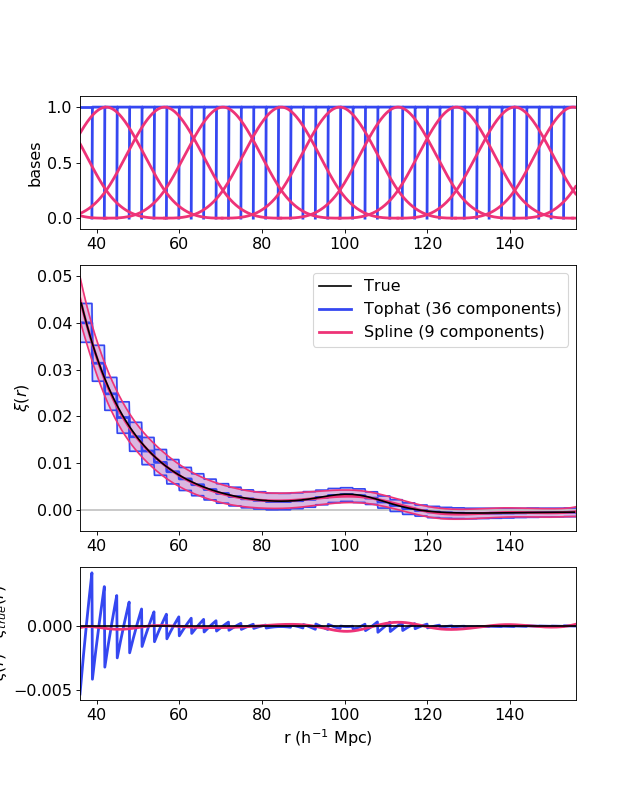
\includegraphics[width=0.8\textwidth]{xicomparison_2e-4_tophat3_spline}
    \caption{A comparison between \est with a cubic spline basis function (red) and the standard tophat estimator (blue). The shaded region is the standard deviation of the \cf estimate of the 1000 mock catalogs. The cubic spline estimator has lower bias and lower variance with fewer bins. \KSF{quote rmse in caption? otherwise not clear from figure its less biased.} \hogg{yes} \KSF{does tophat need to be a different linestyle?}} \KSF{make tophat thin, spline thick, choose thin for black truth} \KSF{change ylim to 0.03} \KSF{restrict error ylim, symmetric +/-}

\end{figure}

A natural extension of tophat basis functions is the B-spline.
B-splines of order $n$ are piecewise polynomials of order $n-1$; they constitute the basis functions for spline interpolation \KSF{CITE}.
They have the nice property that the functions and their derivatives can be continuous, depending on the order.
Further, B-splines are well-localized, which provides a more direct comparison to the typical tophat basis (which is entirely localized).
For this demonstration we use fourth-order B-splines, which constitute the set of basis functions for a cubic spline, as they are the lowest-order spline to have a continuous first derivative.
We compare this standard estimator, reformulated as continuous functions using a tophat basis.
For the tophat basis we use 18 basis functions in the range $36 < r < 144$ \hmpc, each with a width of 6 \hmpc.
This is a standard bin width for two-point analyses. \KSF{cite optimal bin width paper}
For the cubic spline basis, we use the same $r$ range, but with only 9 basis functions, and knots chosen to evenly span this $r$ range with this number of basis functions.

The results are shown in Figure~\ref{fig:spline}.
We can compare our estimation to the known true input \cf, which is the Fourier transform of the input power spectrum.
The spline basis clearly produces a better fit to the true correlation function in its smoothness and accuracy across the scale range.
Even when we compare the error of the estimates at the effective redshift of each bin, as is done in standard practice, our spline basis achieves lower bias and variance \KSF{need plot showing}.
Thus, \est allows for a more accurate and precise estimate of the \cf with fewer components.
\KSF{TODO: elaborate more here}


\subsection{BAO Scale Estimation Test}
\label{sec:bao}

Measurement of the BAO scale provides a good use case for our estimator.
The BAO feature is a peak in clustering on large scales, $\sim$150 Mpc, making it less sensitive to small-scale astrophysical effects.
It is one of the best tools for constraining cosmological models, in particular the distance-redshift relation \citep{Kazin2010, Anderson2012, Anderson2014, Alam2016}.

\KSF{what else do I need to cite for BAO?}

We base our BAO estimation on the method of the BOSS DR10 and 11 analysis \citep{Anderson2014}.
We estimate the spherically averaged 3-dimensional correlation function, $\bld{\hat{\xi}}(r)$, where $r$ is the separation between pairs.
(BAO analyses is typically done in redshift space, estimating $\bld{\hat{\xi}}(s)$, where $s$ is the redshift-space separation between pairs, but here we are using a toy model a periodic box in which we know the true galaxy positions so we just use the real-space distance $r$.)
In order to extract information about the baryon acoustic feature from galaxy clustering, we must choose a fiducial cosmological model to convert redshifts to distances.
If we choose an incorrect model, the scales in the power spectrum will be dilated, so the oscillation wavelength---and thus the BAO peak position---will be shifted.
We can model this shift as a scale dilation parameter, $\alpha$, which is a function of the relevant distance scales in the true and fiducial cosmologies:
\begin{equation} \label{eq:alpha}
\alpha = \Bigg( \frac{D_\mathrm{A}(z)}{D_\mathrm{A}^{\text{mod}}(z)} \Bigg)^{2/3} \Bigg( \frac{H^{\text{mod}}(z)}{H(z)} \Bigg)^{1/3} \Bigg( \frac{r_\mathrm{s}^{\text{mod}}}{r_\mathrm{s}} \Bigg),
\end{equation}
where $D_\mathrm{A}$ is the angular diameter distance, $H$ is the Hubble constant, $r_\mathrm{s}$ is the sound horizon scale at the drag epoch, and the superscript ``$\text{mod}$'' denotes the value for the fiducial model.
Qualitatively, if the fit prefers $\alpha>1$, this suggests the true position of the BAO peak is at a smaller scale than in the fiducial model, whereas if $\alpha<1$, the peak is at a larger scale.

In standard practice, the fitting function used to determine the value of $\alpha$ is
\begin{equation}
\xi^{\mathrm{fit}}(r) = B^2 \xi^{\mathrm{mod}}(\alpha r) + \frac{a_1}{r^2} + \frac{a_2}{r} + a_3
\end{equation}
where $B$ is a constant that allows for a large-scale bias, and $a_1$, $a_2$, and $a_3$ are nuisance parameters to account for the broadband shape.
A $\chi^2$ fit is performed with five free parameters: $\alpha$, $B$, $a_1$, $a_2$, and $a_3$. 
\KSF{TODO: check how this is actually done!}
The resulting value for $\alpha$ is used to derive the actual values of the distance scales of interest.
Typically, density-field reconstruction is performed before applying the estimator to correct for nonlinear growth around the BAO scale \citep{Eisenstein2007}; for our toy example, we will omit this step.

The form of the standard fitting function is well-suited to our estimator, as it is a few-parameter model with a linear combination of terms.
To use our estimator to estimate $\alpha$, we add a term that includes the partial derivative of the model with respect to $\alpha$.
This allows us to have fixed basis functions, and for an initial choice of $\alpha_\mathrm{guess}$, determine the change in this value needed to improve the fit. 
Our fitting function is then
\begin{equation} \label{eq:baoiter_fit}
\xi^\mathrm{fit}(r) = B^2\,\xi^\mathrm{mod}(\alpha_\mathrm{guess}\,r) + C\,k_0\,\frac{\dd \xi^\mathrm{mod}(\alpha_\mathrm{guess}\,r)}{\dd \alpha} + a_1\,\frac{k_1}{r^2} + a_2\,\frac{k_2}{r} + a_3\,k_3 ,
\end{equation}
where $C$ is an additional coefficient that describes the contribution of the derivative term, and $k_0$, $k_1$, $k_2$, and $k_3$ are constants that determine the initial amplitude of the basis functions.
In this case, the free parameters are $B^2$, $C$, $a_1$, $a_2$, and $a_3$.
Note that in theory the choice of $k_i$ values shouldn't matter as the estimator is affine invariant (see Appendix \ref{sec:affine}), but in practice reasonable choices are important for stability.

To use the estimator for a BAO measurement, we input these five terms as the five basis functions of our estimator.
\KSF{update this given the above list of free params}
The estimator outputs an amplitude vector $\bld{a}$ as described in $\S$\ref{sec:est}, which describes the contribution of each basis function---precisely the values of the free parameters.
From the value of $C$, we can determine our estimate of the scale dilation parameter, $\hat{\alpha}$, as $\hat{\alpha} = \alpha_\mathrm{guess} + C\,k_0$. 
With this formulation, a value of $C=0$ indicates that the current $\alpha_\mathrm{guess}$ gives the best fit to the data (given the chosen cosmological model), while nonzero values give the magnitude and direction of the necessary change in the scale dilation parameter.
In practice, we apply an iterative procedure to converge at our best estimate $\hat{\alpha}$; this procedure and other implementation details are described in Appendix \ref{sec:baoiter}.

\label{fig:bao_bases}
\begin{figure}[ht]
\centering
    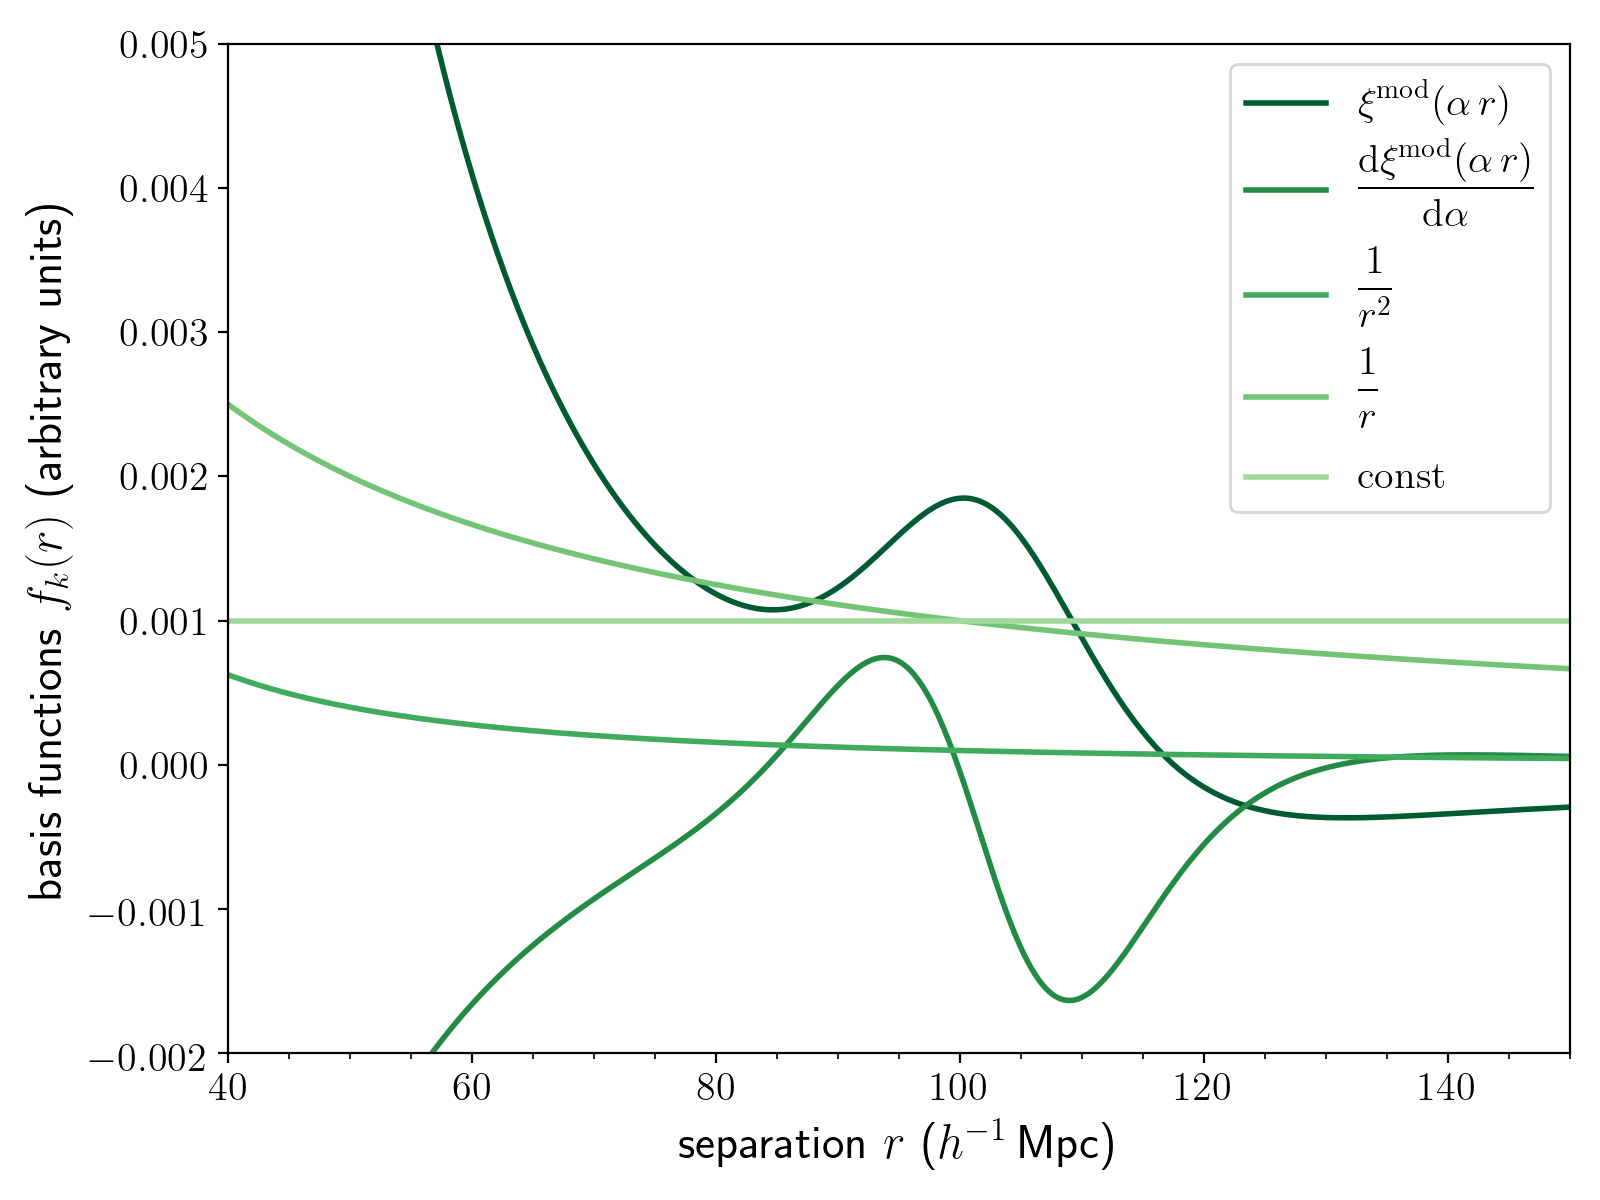
\includegraphics[width=0.8\textwidth]{bao_bases}
    \caption{The set of basis functions used to fit for the BAO scale using our estimator. The $B^2$ term (green) is the fiducial model used to determine the scale dilation parameter $\alpha$. The $C$ term is the derivative of this model with respect to $\alpha$, allowing for the estimation of this parameter. The $a_1$, $a_2$, and $a_3$ terms are nuisance parameters to fit the broadband shape. \KSF{Make colorblind friendly! try diff greens (change alpha?)}} \KSF{fix latex; displaystyle}
\end{figure}

We demonstrate this method using the same set of lognormal mocks as in $\S$\ref{sec:spline}.
We construct a recovery test following that in \cite{Hinton2019}.
We assume the fiducial cosmological model used in \cite{Beutler2017}: $\Omega_{\text{m}} = 0.31$, $h = 0.676$, $\Omega_{\text{b}} = 0.04814$, $n_s = 0.97$. 
As we know the cosmology used for our mock catalogs, we can compute the true value of the scale dilation parameter, $\alpha_{\text{true}}=0.9987$.
(Here our choice of fiducial model happened to be close to the true model, so our $\alpha_{\text{true}}$ is very close to 1; this is typical, as our cosmological model is fairly well-constrained.)
With this fiducial model, we can construct the basis functions for our estimator; these are shown (with $\alpha=1$ and reasonable choices for the scaling parameters $k$) in Figure~\ref{fig:bao_bases}.

We apply our iterative estimation procedure to each of the 1000 mocks; the resulting estimate for the correlation function is shown in Figure~\ref{fig:bao}.
The mean BAO estimate is shown in orange, and the mean tophat estimate is in blue; the truth is in black.
Our estimator clearly better represents the shape of the known \cf.
The mean value of the final recovered scale dilation parameter is $\alpha=XXX \pm YYY$, very close to the true value.

\label{fig:bao}
\begin{figure}[th]
\centering
    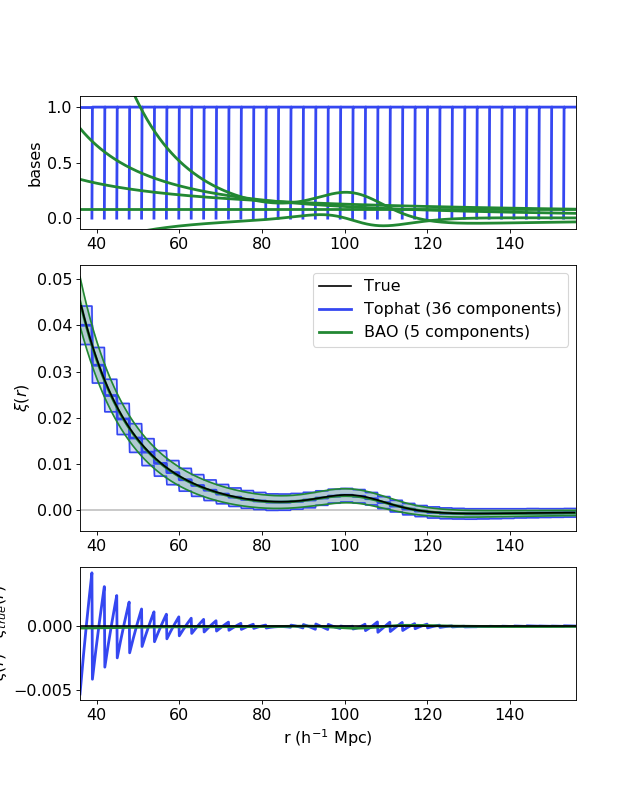
\includegraphics[width=0.8\textwidth]{xicomparison_2e-4_tophat3_baoiter}
    \caption{Estimation of the correlation function using our estimator with basis functions based on the BAO fitting function (orange dot-dashed). The line is the mean of the final estimate from the iteration procedure for 100 mocks, and the shaded region is the $1\sigma$ variation. We also show the standard Landy-Szalay estimator, displayed as a tophat function (blue), as well as the true input correlation function (black). \KSF{This is for the 1e-4 box, need to run bigger box.} \KSF{Should this and the basis set figure be a single figure with two panels?} \KSF{Should i have a figure showing the sum of the basis functions and how that gets you the final cf?}}
\end{figure}

We note that these basis functions are significantly different than the tophat or B-spline bases previously explored, mainly because they are not localized.
This means that data at all scales could contribute to all basis functions.
It is then critical to ensure that the final parameter estimate does not rely on the range of scales chosen.
We have confirmed that in this application, the result is robust to the chosen range as long as the scales cover the range $40<r<200$ \hmpc, the typical range used in BAO analyses. \KSF{Actually have to check this and update numbers!}


\section{Discussion} \label{sec:discuss}

\subsection{Relationship to Other Existing Estimators}
\label{sec:otherest}

\Est has properties similar to existing estimators, including kernel density estimators and the marked correlation function.
With the proper choice of basis functions, \est can indeed produce both of these estimators; it is more general than either of them.

Kernel density estimation (KDE) is a class of methods for estimating a probability density function from a set of data.
KDE methods essentially smooth the data with a given kernel, often a Gaussian.
\KSF{should i cite the original KDE papers from the 50s and 60s? or not necessary bc not the focus?}
This is useful when we want to reconstruct a distribution without making many assumptions about the data, as is required in parametric methods.
KDEs have found use in many areas of astrophyics, for example to measure the 21cm power spectrum with reduced foreground contamination \citep{Trott2019}, and to estimate luminosity functions with superior performance compared to binned methods \citep{Yuan2020}.
\KSF{there are others, should i list more citations? without describing?}
\cite{Hatfield2016} uses a KDE approach to estimate the angular correlation function, in order to address the issues of information loss and arbitrary bin choice inherent to binning; they optimize for the kernel choice, and find a correlation function consistant with that of the binned method.
\KSF{I couldnt find any other papers that use KDEs on correlation functions, but i found this one by chance. more to say here? the paper doesn't draw strong conclusions from this.}

Specifically, kernel density estimators take the contribution of each data point to be a kernel function centered on that value, and sum these to determine the full distribution.
In contrast, \est projects each data point onto fixed basis functions, which are distinct from the typical understanding of kernels.
As such, our estimator is not smearing out the data, as KDEs do; it is using the data to directly infer the contribution of each basis function.
This preserves the information in the data to the degree given by the chosen set of basis functions, which can in fact enhance features rather than smooth them.
That said, the formulation of \est is general enough that it can perform a kernel density estimate of the correlation function, by choosing $f(r)$ to be a kernel centered on $r$.
However, our uses here of the estimator are fundamentally different from KDE methods, as they use use fixed basis functions that can take advantage of the science use case and preserve maximal information from the data.
\KSF{this last sentence is a bit repetitive / are there more differences im missing?}

\KSF{Paragraph on marked cf}

\label{ref:beyondls}
\subsection{Beyond the Landy-Szalay Estimator}

While we have formulated our estimator as a generalization of \LS, as it is the standard used in \cf analyses and has optimal properties under certain conditions, we can also reformulate it for other estimators.
Our formulation currently requires a normalization term (i.e. denominator) of the $\vv{RR}$ counts, as we replace this with our $\TT{RR}$ term.
This is the case for the \cite{PeeblesHauser1974} (natural) estimator and the \cite{Hewett1982} estimator:
\begin{eqnarray}
    \xi_{PH} &=& \frac{\vv{DD} - \vv{RR}}{\vv{RR}} \rightarrow \TT{RR}\inv \cdot \left( \vv{DD} - \vv{RR} \right)\\
    \xi_{Hew} &=& \frac{\vv{DD} - \vv{DR}}{\vv{RR}} \rightarrow \TT{RR}\inv \cdot \left( \vv{DD} - \vv{DR} \right).
\end{eqnarray}
We can also generalize estimators which have a $\vv{DR}$ cross-correlation term as the denominator, such as the \cite{DavisPeebles1983} estimator,
\begin{equation}
    \xi_{DP} = \frac{\vv{DD} - \vv{DR}}{\vv{DR}} \rightarrow \TT{DR}\inv \cdot \left( \vv{DD} - \vv{DR} \right)
\end{equation}
by defining
\begin{equation}
    \TT{DR} = \frac{2}{\NN{D}\,\NN{R}} \sum_{n} \sum_{m} \ff(\GG{n}, \GG{m}) \cdot \ff\T(\GG{n}, \GG{m}).
\end{equation}
This could be extended to nearly any linear combination of pair counts.
The estimator of \cite{VargasMagana2013} selects the optimal combination of pair counts; our estimators could be combined to create an even more generalized estimator.
\KSF{some of the terms in V-M include DD in the denom - need to mention this?}
\KSF{what about estimator with DRsquared in the denom (hamilton estimator?) as trivial as naive guess?}

\KSF{havent updated; think i will be able to delete this paragraph once i nail down the prefactors for the estimator}
We also note that the \est can be easily generalized to cross-correlations between two datasets.
In this case, we consider datasets $D_1$ and $D_2$, and associated random catalogs $R_1$ and $R_2$. 
We then have two different data-random terms, crossing each dataset with the opposite random catalog, resulting in a \LS estimator of the form
\KSF{notation is now clunky with double subscripts; could make 1 and 2 superscript? or maybe it's fine with the parens}
\begin{equation}
    \hat{\xi}_k = \frac{(D_1 D_2)_k - (D_1 R_2)_k - (D_2 R_1)_k + (R_1 R_2)_k}{(R_1 R_2)_k}.
\end{equation}
Here, each term is normalized simply by the number of pairs, as
\begin{equation}
    D_1 D_2 \equiv \frac{1}{N_{D1} N_{D2}} \sum_{n n'} f(T_n, T_{n'})
\end{equation}
and similarly for the other terms.
This cross-correlation formulation can be extended to other estimators beyond \LS in a straightforward way.

\subsection{Computational Performance}

The computational scaling is by definition the same as traditional estimators, because pair-finding remains the limiting factor.
\Est has the additional need for evaluating the function $f$ for each pair of galaxies.
For simple basis functions like splines, this will only marginally decrease performance.
For more complicated functions such as evaluating a cosmological model, \est may incur extra computational expense.
Basis functions can also be input on a grid and then interpolated; the performance is then the same for all functions, but the interpolation for each function for each pair does somewhat decrease the performance.

\KSF{Is there a need to say much more? If not, maybe doesn't deserve its own section - could this go in the implementation section? Or maybe tacked onto another small section if we have one that makes sense}
\KSF{where to put other implemenation notes? e.g. using DD(s,mu) for realspace cf, with 1 big mu bin.}

\subsection{Effect on Covariance Matrix Estimation}

We have shown that \est results in \cf estimates that are just as accurate with fewer components.
This is critical when estimating the covariance matrix, which is necessary for parameter inference.
The covariance matrix is difficult to compute theoretically;instead, it is usually estimated by evaluating the \cf on a large number of mock catalogs and computing the covariance between the bins (e.g. \citealt{Reid2010}; \citealt{Anderson2014}).
The unbiased estimator for the sample covariance matrix is (e.g. \citealt{Anderson2003})
\KSF{index notation getting clunky, thoughts?}
\begin{equation}
\bld{\hat{C}}^\mathrm{ML}_{ij} = \frac{1}{\NN{mocks}-1} \sum_{q=1}^{\NN{mocks}} \left( \left[\bld{\xi}_q \right]_i - \bar{\bld{\xi}}_i \right) \left( \left[\bld{\xi}_q \right]_j - \bar{\bld{\xi}}_j \right),
\end{equation}
where $q$ denotes the index of the mock, $i$ and $j$ denote the index of the bin or component, $\bld{\xi}$ denotes the estimate in that bin for that mock, and $\bar{\bld{\xi}}$ denotes the mean value of the estimate in that bin across the mocks, where we have omitted the hat for clarity. \KSF{i removed the hats here because they didn't play nicely w the average bar; thoughts?}
To get an unbiased estimate of the inverse covariance matrix, we require a correction factor, as the inverse of an unbiased estimator is not necessarily unbiased.
The unbiased estimator for the sample inverse covariance matrix can be shown to be \citep{Hartlap2007}
\begin{equation}
\bld{\hat{C}}\inv = \frac{\NN{mocks}-\NN{bins}-2}{\NN{mocks}-1} \left( \bld{\hat{C}}^\mathrm{ML} \right) \inv.
\end{equation}

%This prefactor correction results in the  propagates to the variance in 
The variance in the elements of this estimator then have a dependence on $\NN{mocks}$ and $\NN{bins}$.
This propagates to the derived cosmological parameters, resulting in an overestimation of the error bars (\citealt{Hartlap2007}; \citealt{Dodelson2013} \citealt{Percival2014}; \citealt{TaylorJoachimi2014}).
Assuming that $\NN{mocks} >> \NN{bins}$ (and both much larger than the number of parameters to be estimated), and that the measurements are Gaussian distribued, the error bars are inflated by a factor of $(1 + \NN{bins}/\NN{mocks})$ (i.e., the true constraints are tighter than the derived ones).
This factor becomes critical at the precision of cosmological parameter estimation \citep{Percival2014}.

Typically, this is dealt with by generating a very large number of mocks.
For the Baryon Oscillation Spectroscopic Survey (BOSS, \citealt{Dawson2013}), $\sim$600 mocks were needed and the analysis used 41 bins \citep{Sanchez2012}.
Future surveys will have more costly requirements on mock catalogs, with larger simulations necessary to cover the larger survey volumes.

An alternative to increasing $\NN{mocks}$ is decreasing $\NN{bins}$ to achieve the same error on precision.
In the standard method, this is shown to \emph{increase} the statistical error, albeit only slightly \cite{Percival2014}.
A substantial increase in bin width would prevent capturing information in finer clustering features; even the relatively broad BAO peak requires a bin size on the order of its width of $\sim$10\hmpc.
In fact, in the standard method more bins would typically be desireable, but the number is limited by the available number of mocks for covariance matrix computation.

With our estimator, we have shown that we can reduce the variance by using fewer components, without sacrificing accuracy.
This means that we can safely reduce $\NN{bins}$, or in our replacement of bins with continuous functions, the number of basis functions $K$.
The covariance matrix will be the covariance between these basis functions. \KSF{worth noting that the structure of this covmat will be significantly different, esp if non-orthogonal?}
To then achieve the same precision on the error on the cosmological parameters, a lower value of $\NN{mocks}$ becomes possible.
This will significantly reduce requirements on mocks, which will be particularly important for upcoming large surveys. 

\KSF{I think the result of discussions was that there wasn't a good way of showing this without propagating all the way to cosmological parameters. Would love a figure showing lower covariance errors but not sure how without full propagation}

\subsection{Further Applications}

The formulation of \est opens up many possibilities for extracting information from the correlation function.
The most straightforward applications are standard basis functions or linearizeable astrophysical models, as we have shown here.
Other applications for the direct estimation of cosmological parameters could include the growth rate of cosmic structure $f$ \citep{Satpathy2016, Reid2018} and primordial non-Gaussianity in the local density field $f^{local}_{NL}$ \citep{Karagiannis2014}.
\KSF{mention idea of doing full cosmo model analysis by taking derivs wrt cosmological params? cool but less connected to citeable papers perhaps}

We can take our estimator a step further by choosing basis functions that depend not only on the separation between tracer pairs, but also on the properties of the tracers themselves.
One such application is the redshift dependence of the Alcock-Paczynski effect \cite{AlcockPaczynski1979}, which can be used to constrain the matter density $\Omega_m$ and the dark energy equation of state parameter $w$ \citep{Li2016}.
The basis functions $f$ in this case would take the form
\begin{equation}
    \ff_k(\GG{n}, \GG{n'}) = \ff_k(|\bld{r}_n - \bld{r}_{n'}|, z_n, z_{n'}),
\end{equation}
where $z$ is the redshift of tracer $n$ or $n'$.
Another potential use case is the luminosity and color dependence of galaxy clustering, which can be used to understand the relationship between galaxy formation and the LSS \citep{Zehavi2011}.
This could be extended to other galaxy properties.

The estimator gives us the opportunity to investigate more subtle or exotic signals which are anomalous with respect to our conventional models.
Anomalies could appear as inhomogeneities or anisotropies in the data.
For example, cosmological parameters could vary across the sky, which has previously investigated in patches across the Cosmic Microwave Background \citep{MukherjeeWandelt2018}.
Another possibility is anisotropy in the cosmic acceleration, which could leave signatures in measurements made using various phenomena including baryon acoustic oscillations \citep{Faltenbacher2012} and Type Ia supernovae \citep{Colin2019}.
With our estimator, we could introduce a dependence on location or direction into our basis functions, and constrain the potential deviation from homogeneity or isotropy.
While these effects would be highly degenerate with systematics, our estimator combined with robust systematics mitigation allows us to investigate the possibility of new physics.

Finally, our estimator can be directly related to a power spectrum analysis.
We could use a Fourier basis as our set of continuous functions.
This would allow us to directly project the data onto Fourier modes.
This represents a step towards unifying the correlation function and the power spectrum. \KSF{there's more to say here but I'm not sure what}


\section{Summary}

\KSF{TODO: write short summary}

\acknowledgements
KSF was supported by the NASA FINESST grant [grant number] during the completion of this work.
The authors thank Jeremy Tinker and Michael Blanton for helpful discussions, Roman Scoccimarro for insightful conversation, and the members of the Flatiron Astronomical Data Group for useful feedback.
KSF would like to acknowledge significant code feedback and support from Manodeep Sinha, as well as Lehman Garrison.
KSF thanks Drew Jamieson, Chris Lovell for helpful discussion...
All of the code used in this paper is available open-source at \texttt{github.com/kstoreyf/Corrfunc} and \texttt{github.com/kstoreyf/continuous-estimator}. 

\appendix
\section{Affine Invariance}\label{sec:affine}

The estimator is invariant under an affine transformation, meaning that the estimate of the \cf will be equivalent under rescalings or stretches. \KSF{check/reword this}
We represent the affine transformation by a transformation matrix $\bld{M}$ that modifies the basis functions $\ff$, such that 
\begin{equation}
\ff' \leftarrow \bld{M}\,\ff
\end{equation}
where the prime indicates our affine-transformed basis.
\KSF{im also using primes for indices, looks a bit confusing; another notation for this?}
Then in the primed basis, the pair counts become
\KSF{double sum? align w choice in sec 2}
\KSF{equal or equivalent? (2 or 3 lines)}
\begin{eqnarray}\displaystyle
\vv{DD}' &=& \sum_{n n'} \ff_{n n'}' = \sum_{n n'} \bld{M}\,\ff_{n n'} = \bld{M}\,\vv{DD}
\\
\vv{DR}' &=& \sum_{n m} \ff_{n m}' = \sum_{n m} \bld{M}\,\ff_{n m} = \bld{M}\,\vv{DR}
\\
\vv{RR}' &=& \sum_{m m'} \ff_{m m'}' = \sum_{m m'} \bld{M}\,\ff_{m m'} = \bld{M}\,\vv{RR}
\end{eqnarray}
where we use the shorthand $\ff_{i j} = \ff(\GG{i}, \GG{j})$ and we have omitted the normalization factors for simplicity.
In the last step, we have factored $\bld{M}$ out of the summation and written the primed vectors in terms of the unprimed vectors. 

For the random-random tensor we have
\begin{eqnarray}\displaystyle
\TT{RR}' &=& \sum_{m m'} (\bld{M}\,\ff_{m m'}) \cdot (\bld{M}\,\ff_{m m'})\T \\
&=& \bld{M}\left[ \sum_{m m'} \ff_{m m'} \cdot \ff_{m m'}\T \right] \bld{M}\T \\
&=& \bld{M}\,\TT{RR}\,\bld{M}\T
\end{eqnarray}
Then the amplitudes in the primed basis become
\begin{eqnarray}\displaystyle
\bld{a}' &=& \TT{RR}\invp \cdot (\vv{DD}' - 2\,\vv{DR}' + \vv{RR}') \\
\bld{a}' &=& [\bld{M} \TT{RR} \bld{M}\T]\inv \cdot [\bld{M}\,\vv{DD} - 2\,\bld{M}\,\vv{DR} + \bld{M}\,\vv{RR}] \\
&=& (\bld{M}\T)\inv \, \TT{RR}\inv \, \bld{M}\inv \cdot \bld{M}\,[\vv{DD} - 2\,\vv{DR} + \vv{RR}] \\
&=& (\bld{M}\T)\inv \, \TT{RR}\inv \cdot [\vv{DD} - 2\,\vv{DR} + \vv{RR}] \\
&=& (\bld{M}\T)\inv \, \bld{a}
\end{eqnarray}
and the estimator $\bld{\hat{\xi}}'$ in the primed basis, where we are again using the shorthand $\bld{\hat{\xi}} = \bld{\hat{\xi}}(\GG{i}, \GG{j})$, is 
\begin{eqnarray}\displaystyle
\bld{\hat{\xi}}' &=& \bld{a}\Tp \cdot \ff \\
\bld{\hat{\xi}}' &=& [(\bld{M}\T)\inv \, \bld{a}]\T \cdot (\bld{M}\,\ff) \\
&=& \bld{a}\T \, [(M\inv)\T]\T \cdot (\bld{M}\,\ff) \\
&=& \bld{a}\T \, \bld{M}\inv \cdot \bld{M}\,\ff \\
&=& \bld{a}\T \cdot \ff \\
&=& \bld{\hat{\xi}}.
\end{eqnarray}
Thus after an affine transformation of the basis function, the resulting estimator is equivalent to the estimator in the original basis.

We note that this requires $\bld{M}$ be invertible.
However, any two equivalent bases must be related by the inverse of a transformation matrix, so this requirement is already satisfied.
\KSF{I don't understand what i wrote here. what more to say about this?}


\section{Computing the Random-Random Terms Analytically}\label{sec:analytic}

The autocorrelation of the random catalog is meant to approximate the window function. 
When we have a periodic cube, we can compute this $\vv{RR}$ term analytically.
Here we derive this, and then derive the equivalent for our continuous-basis $\vv{RR}$ and $\TT{RR}$ terms.

Our goal is to estimate the number of pairs in a periodic cubic volume filled uniformly with tracers, $\vv{RR}^\mathrm{ana}$. 
We first consider an annulus indexed by $k$ around a single galaxy, with radial edges $g_k$ and $h_k$. 
This annulus has a volume $V_k$.
Taking the box to have an average number density $\bar{n}$, the number of galaxies expected in the annulus is $N_k = V_k \bar{n}$, and thus our selected galaxy contributes $N_k$ pairs to the count.   
\KSF{do i put mathspaces between multiplications when there's already a parenthesis?}
We do this for each of the $\NN{D}-1$ other galaxies, and after including a factor of $\frac{1}{2}$ accounts for the fact that this double-counts pairs, we find a total pair count of $\left[ \vv{RR}^\mathrm{ana} \right]_k = \frac{1}{2}(\NN{D}-1) N_k = \frac{1}{2}(\NN{D}-1) V_k \bar{n}$.
For a cubic volume, $\bar{n} = \NN{D}/L^3$, so our final pair count for the annulus is 
\begin{equation}
\left[ \vv{RR}^\mathrm{ana} \right]_k = \frac{1}{2} \frac{\NN{D}}{L^3} (\NN{D}-1) V_k.
\end{equation}

We next need to compute $V_k$; for hard-edged radial bins, we can compute $V_k$ simply as the difference between spherical volumes. 
We can represent this more generally as an integral,
\begin{equation} \label{eq:vol_tophat}
V_k = \int_{g_k}^{h_k} dV = 4\pi \int_{g_k}^{h_k} r^2 dr.
\end{equation}
We can easily generalize this to any basis function $\ff_k(r)$ that is only a function of $r$,
\begin{equation}
V_k = 4\pi  \int_{g_k}^{h_k} \ff_k(r) r^2 dr
\end{equation}
where $k$ is now the index of the basis functions.
We can see that this reduces to Equation \ref{eq:vol_tophat} when $\ff(r)$ is the tophat function (returning 1 or 0 depending on whether or not $r$ falls between $g_k$ and $h_k$).

Combining the above equations gives us our full generalized analytic random-random vector $\vv{RR}^\mathrm{ana}$, which has elements
\begin{equation}
\left[ \vv{RR}^\mathrm{ana} \right]_k = \frac{1}{2} \, \frac{\NN{D}}{L^3} \,(\NN{D}-1) \, 4\pi \, \int_{0}^{r_\mathrm{max}} \ff_k(r) \, r^2 \, dr
\end{equation}
where we are now integrating over all values of $r$ we are interested in (from 0 out to some $r_\mathrm{max}$), to account for non-localized basis functions. 

Based on the definition of $\TT{RR}$ in Equation \ref{eq:qq_proj} as the outer product of the basis function vector and its transpose, we can see that the elements of the analytic random-random tensor $\TT{RR}^\mathrm{ana}$ can be written as
\begin{equation}
\left[ \TT{RR}^\mathrm{ana} \right]_{kk'} = \frac{1}{2} \, \frac{\NN{D}}{L^3} (\NN{D}-1) \, 4\pi \, \int_{0}^{r_\mathrm{max}} \ff_k(r) \, \ff_{k'}(r) \, r^2 \, dr
\end{equation}
This could be further generalized to account for basis functions that take other properties as input.

When considering a periodic box, the natural estimator is no longer biased, so we can also avoid computing the cross-correlation term $\vv{DR}$ and calculate the amplitudes as 
\begin{equation}
\bld{a}_{\mathrm{ana}} = \left[ \TT{RR}^\mathrm{ana} \right]\inv \cdot \vv{DD}.
\end{equation}
Looking back, it might have seemed strange that we use $\NN{D}$ in calculating the analytical term $\vv{RR}^\mathrm{ana}$, but we now see that this normalization prefactor cancels out with that of the $\vv{DD}$ term.
Finally, we use these amplitudes $\bld{a}_{\mathrm{ana}}$ to compute the correlation function $\bld{\hat{\xi}}_{\mathrm{ana}}$ as before in Equation \ref{eq:xi_proj}.

\section{Implementation of Estimation with BAO Basis Functions}\label{sec:baoiter}

\subsection{Iterative Procedure}
\Est can be used to measure the baryon acoustic oscillation (BAO) scale by choosing the basis functions to terms of a BAO fitting function, as described in \ref{sec:bao}.
For this application, we need to choose a fiducial cosmology for our bases, which will be offset from the true cosmology.
This offset can be encoded by a scale dilation parameter $\alpha$, which contains the information about the BAO scale; see Equation \ref{eq:alpha}. 
As our fitting function requires a fiducial model and an initial guess of this parameter, $\alpha_\mathrm{guess}$, and then determines the change needed, an iterative procedure is needed to converge to the best-fit value.

We start with assuming that we have chosen our fiducial model to match our true cosmology (we in all likelihood have not, but it's not a bad initial guess), giving us an initial $\alpha_\mathrm{guess} = 1.0$. 
We then apply \est to perform the measurement, and obtain the amplitude $C$ for the derivative term in our model as in Equation \ref{eq:baoiter_fit}. 
This gives us our estimate $\hat{\alpha}$ of the scale dilation parameter from this initial model; for the $i$th iteration, we have
\begin{equation}
    \hat{\alpha}_{i} = \alpha_{\mathrm{guess},i} + C_i \, k_0
\end{equation}
where $k_0$ is the chosen scaling parameter for the derivative basis function as in Equation \ref{eq:baoiter_fit}.

We choose the convergence criterion to be when the fractional change in $\hat{\alpha}$ between subsequent iterations falls below a threshold, $c_\mathrm{thresh}$ \KSF{name for this variable?},
\begin{equation}
    \left| \frac{\hat{\alpha}_i - \hat{\alpha}_{i-1}}{\hat{\alpha}_i} \right| < c_\mathrm{thresh}.
\end{equation}
For our application we choose $c_\mathrm{thresh} = 0.00001$.

To achieve convergence, we need to be careful in choosing our next $\alpha_{\mathrm{guess},i}$.
If it is far from the best estimate, $C_i$ will be large, and our resulting estimate $\hat{\alpha}_{i}$ will be inaccurate.
We thus include a damping parameter $\eta$ between 0 and 1 to improve our convergence.
Our next guess is then
\KSF{what should the assignment symbol be here?}
\begin{equation}
    \alpha_{\mathrm{guess},i+1} \leftarrow \alpha_{\mathrm{guess},i} + \eta\,C_i\,k_0.
\end{equation}
The choice of $\eta$ is important for stability and speed of convergence; too large a value can lead to a back-and-forth cycle in which the result hops between two values and never converges, and too small a value would make convergence take a very long time.
In our application, we start with $\eta=0.5$.
We check if our estimate is jumping over the true value by checking if the error changes sign; if it does, we reduce $\eta$ by a factor of $0.75$.

\subsection{Implementation Details}

We implement the partial derivative in the fitting function as a finite difference between model with the our chosen value of $\alpha_\mathrm{guess}$, and the model with a value shifted by a small $\Delta \alpha$,
\KSF{what should the assignment symbol be here?}
\begin{equation}
    \frac{\dd \xi^\mathrm{mod}(\alpha s)}{\dd \alpha} \leftarrow \frac{\xi^\mathrm{mod}(\alpha_\mathrm{guess} s) - \xi^\mathrm{mod}((\alpha_\mathrm{guess} + \Delta \alpha)s)}{\Delta \alpha}.
\end{equation}
In our implemenation we take $\Delta \alpha = 0.001$; we check that our results are insensitive to this choice.

We choose the amplitudes of the basis functions $k$ to set them at similar scales.
We use $k_0=0.1$, $k_1=10.0$, $k_2=0.1$, and $k_3=0.001$.

%need style file error
%\bibliographystyle{apj} 
%\bibliography{paper}
% To copy from mendeley locally: in paper dir, [cp ~/code/bibtex/LSS-est_paper.bib .]
\bibliography{LSS-est_paper}

\end{document}














